% Options for packages loaded elsewhere
\PassOptionsToPackage{unicode}{hyperref}
\PassOptionsToPackage{hyphens}{url}
%
\documentclass[
]{article}
\usepackage{amsmath,amssymb}
\usepackage{lmodern}
\usepackage{iftex}
\ifPDFTeX
  \usepackage[T1]{fontenc}
  \usepackage[utf8]{inputenc}
  \usepackage{textcomp} % provide euro and other symbols
\else % if luatex or xetex
  \usepackage{unicode-math}
  \defaultfontfeatures{Scale=MatchLowercase}
  \defaultfontfeatures[\rmfamily]{Ligatures=TeX,Scale=1}
\fi
% Use upquote if available, for straight quotes in verbatim environments
\IfFileExists{upquote.sty}{\usepackage{upquote}}{}
\IfFileExists{microtype.sty}{% use microtype if available
  \usepackage[]{microtype}
  \UseMicrotypeSet[protrusion]{basicmath} % disable protrusion for tt fonts
}{}
\makeatletter
\@ifundefined{KOMAClassName}{% if non-KOMA class
  \IfFileExists{parskip.sty}{%
    \usepackage{parskip}
  }{% else
    \setlength{\parindent}{0pt}
    \setlength{\parskip}{6pt plus 2pt minus 1pt}}
}{% if KOMA class
  \KOMAoptions{parskip=half}}
\makeatother
\usepackage{xcolor}
\usepackage[margin=1in]{geometry}
\usepackage{color}
\usepackage{fancyvrb}
\newcommand{\VerbBar}{|}
\newcommand{\VERB}{\Verb[commandchars=\\\{\}]}
\DefineVerbatimEnvironment{Highlighting}{Verbatim}{commandchars=\\\{\}}
% Add ',fontsize=\small' for more characters per line
\usepackage{framed}
\definecolor{shadecolor}{RGB}{248,248,248}
\newenvironment{Shaded}{\begin{snugshade}}{\end{snugshade}}
\newcommand{\AlertTok}[1]{\textcolor[rgb]{0.94,0.16,0.16}{#1}}
\newcommand{\AnnotationTok}[1]{\textcolor[rgb]{0.56,0.35,0.01}{\textbf{\textit{#1}}}}
\newcommand{\AttributeTok}[1]{\textcolor[rgb]{0.77,0.63,0.00}{#1}}
\newcommand{\BaseNTok}[1]{\textcolor[rgb]{0.00,0.00,0.81}{#1}}
\newcommand{\BuiltInTok}[1]{#1}
\newcommand{\CharTok}[1]{\textcolor[rgb]{0.31,0.60,0.02}{#1}}
\newcommand{\CommentTok}[1]{\textcolor[rgb]{0.56,0.35,0.01}{\textit{#1}}}
\newcommand{\CommentVarTok}[1]{\textcolor[rgb]{0.56,0.35,0.01}{\textbf{\textit{#1}}}}
\newcommand{\ConstantTok}[1]{\textcolor[rgb]{0.00,0.00,0.00}{#1}}
\newcommand{\ControlFlowTok}[1]{\textcolor[rgb]{0.13,0.29,0.53}{\textbf{#1}}}
\newcommand{\DataTypeTok}[1]{\textcolor[rgb]{0.13,0.29,0.53}{#1}}
\newcommand{\DecValTok}[1]{\textcolor[rgb]{0.00,0.00,0.81}{#1}}
\newcommand{\DocumentationTok}[1]{\textcolor[rgb]{0.56,0.35,0.01}{\textbf{\textit{#1}}}}
\newcommand{\ErrorTok}[1]{\textcolor[rgb]{0.64,0.00,0.00}{\textbf{#1}}}
\newcommand{\ExtensionTok}[1]{#1}
\newcommand{\FloatTok}[1]{\textcolor[rgb]{0.00,0.00,0.81}{#1}}
\newcommand{\FunctionTok}[1]{\textcolor[rgb]{0.00,0.00,0.00}{#1}}
\newcommand{\ImportTok}[1]{#1}
\newcommand{\InformationTok}[1]{\textcolor[rgb]{0.56,0.35,0.01}{\textbf{\textit{#1}}}}
\newcommand{\KeywordTok}[1]{\textcolor[rgb]{0.13,0.29,0.53}{\textbf{#1}}}
\newcommand{\NormalTok}[1]{#1}
\newcommand{\OperatorTok}[1]{\textcolor[rgb]{0.81,0.36,0.00}{\textbf{#1}}}
\newcommand{\OtherTok}[1]{\textcolor[rgb]{0.56,0.35,0.01}{#1}}
\newcommand{\PreprocessorTok}[1]{\textcolor[rgb]{0.56,0.35,0.01}{\textit{#1}}}
\newcommand{\RegionMarkerTok}[1]{#1}
\newcommand{\SpecialCharTok}[1]{\textcolor[rgb]{0.00,0.00,0.00}{#1}}
\newcommand{\SpecialStringTok}[1]{\textcolor[rgb]{0.31,0.60,0.02}{#1}}
\newcommand{\StringTok}[1]{\textcolor[rgb]{0.31,0.60,0.02}{#1}}
\newcommand{\VariableTok}[1]{\textcolor[rgb]{0.00,0.00,0.00}{#1}}
\newcommand{\VerbatimStringTok}[1]{\textcolor[rgb]{0.31,0.60,0.02}{#1}}
\newcommand{\WarningTok}[1]{\textcolor[rgb]{0.56,0.35,0.01}{\textbf{\textit{#1}}}}
\usepackage{graphicx}
\makeatletter
\def\maxwidth{\ifdim\Gin@nat@width>\linewidth\linewidth\else\Gin@nat@width\fi}
\def\maxheight{\ifdim\Gin@nat@height>\textheight\textheight\else\Gin@nat@height\fi}
\makeatother
% Scale images if necessary, so that they will not overflow the page
% margins by default, and it is still possible to overwrite the defaults
% using explicit options in \includegraphics[width, height, ...]{}
\setkeys{Gin}{width=\maxwidth,height=\maxheight,keepaspectratio}
% Set default figure placement to htbp
\makeatletter
\def\fps@figure{htbp}
\makeatother
\setlength{\emergencystretch}{3em} % prevent overfull lines
\providecommand{\tightlist}{%
  \setlength{\itemsep}{0pt}\setlength{\parskip}{0pt}}
\setcounter{secnumdepth}{-\maxdimen} % remove section numbering
\ifLuaTeX
  \usepackage{selnolig}  % disable illegal ligatures
\fi
\IfFileExists{bookmark.sty}{\usepackage{bookmark}}{\usepackage{hyperref}}
\IfFileExists{xurl.sty}{\usepackage{xurl}}{} % add URL line breaks if available
\urlstyle{same} % disable monospaced font for URLs
\hypersetup{
  pdftitle={pstat274\_hw02\_aoxu},
  pdfauthor={AO XU},
  hidelinks,
  pdfcreator={LaTeX via pandoc}}

\title{pstat274\_hw02\_aoxu}
\author{AO XU}
\date{2022-10-10}

\begin{document}
\maketitle

\hypertarget{problem-1}{%
\section{Problem 1}\label{problem-1}}

E is correct, data set I and II exhibit statistically significant
autocorrelations since k \(\neq\) 0 and p \textgreater{} 1.

\hypertarget{problem-2}{%
\section{Problem 2}\label{problem-2}}

\hypertarget{a}{%
\subsection{(a)}\label{a}}

It's stationary but not invertible.

It follows MA(2) Module, so it's stationary.

From R, we could get \(B_1\) = 1, \(B_2\) = -3; Since \(B_1\) = 1 lies
on the unit circle, it is not invertible.

\begin{Shaded}
\begin{Highlighting}[]
\FunctionTok{polyroot}\NormalTok{(}\FunctionTok{c}\NormalTok{(}\DecValTok{1}\NormalTok{,}\SpecialCharTok{{-}}\DecValTok{2}\SpecialCharTok{/}\DecValTok{3}\NormalTok{,}\SpecialCharTok{{-}}\DecValTok{1}\SpecialCharTok{/}\DecValTok{3}\NormalTok{))}
\end{Highlighting}
\end{Shaded}

\begin{verbatim}
## [1]  1+0i -3+0i
\end{verbatim}

\hypertarget{b}{%
\subsection{(b)}\label{b}}

It's not stationary but invertible.

It's AR(2) module, and it could converts to (1 - \(\frac{2B}{3}\) -
\(\frac{B^2}{3}\)) \(X_t\) = \(Z_t\). It's invertible since we could
write it as the form of ``\(Z_t\) = \(\phi\)B\(X_t\)''.

From R, we could get \(B_1\) = 1, \(B_2\) = -3; Since \(B_1\) = 1 lies
on the unit circle, it is not stationary.

\begin{Shaded}
\begin{Highlighting}[]
\FunctionTok{polyroot}\NormalTok{(}\FunctionTok{c}\NormalTok{(}\DecValTok{1}\NormalTok{,}\SpecialCharTok{{-}}\DecValTok{2}\SpecialCharTok{/}\DecValTok{3}\NormalTok{,}\SpecialCharTok{{-}}\DecValTok{1}\SpecialCharTok{/}\DecValTok{3}\NormalTok{))}
\end{Highlighting}
\end{Shaded}

\begin{verbatim}
## [1]  1+0i -3+0i
\end{verbatim}

\hypertarget{problem-3}{%
\section{Problem 3}\label{problem-3}}

\hypertarget{a-1}{%
\subsection{(a)}\label{a-1}}

MA(3), \(\theta_1\) = 2, \(\theta_2\) = 0.5, \(\theta_3\) = -0.1

\begin{enumerate}
\def\labelenumi{(\arabic{enumi})}
\item
  The mathematical equation for MA(3) model: \(X_t\) = \(Z_t\) +
  2\(Z_{t-1}\) + 0.5\(Z_{t-2}\) - 0.1\(Z_{t-3}\)
\item
  By using the formula ``\(\rho_x(k)\) =
  \(\frac{\theta_k+\theta_1\theta_{k+1}+...+\theta_{q-k}\theta_k}{1+\theta_1^2+...+\theta_q^2}\)),
  k = 1,2,\ldots,q, \(\rho_x(k)\) = 0, k \textgreater{} q'', we get
\end{enumerate}

\(\rho(1)\) =
\(\frac{\theta_1+\theta_1\theta_2+\theta_2\theta_3}{1+\theta_1^2+\theta_2^2+\theta_3^2}\)
= \(\frac{2+2*0.5+0.5(-0.1)}{1+2^2+0.5^2+(-0.1)^2}\) = 0.56083650

\(\rho(2)\) =
\(\frac{\theta_2+\theta_1\theta_3}{1+\theta_1^2+\theta_2^2+\theta_3^2}\)
= \(\frac{0.5+2(-0.1)}{1+2^2+0.5^2+(-0.1)^2}\) = 0.05703422

\(\rho(3)\) = \(\frac{theta_3}{1+\theta_1^2+\theta_2^2+\theta_3^2}\) =
\(\frac{-0.1}{1+2^2+0.5^2+(-0.1)^2}\) = -0.01901141

\(\rho(4)\) = 0

\begin{Shaded}
\begin{Highlighting}[]
\FunctionTok{ARMAacf}\NormalTok{(}\AttributeTok{ma =} \FunctionTok{c}\NormalTok{(}\DecValTok{2}\NormalTok{, }\FloatTok{0.5}\NormalTok{, }\SpecialCharTok{{-}}\FloatTok{0.1}\NormalTok{), }\AttributeTok{lag.max =} \DecValTok{4}\NormalTok{, }\AttributeTok{pacf =} \ConstantTok{FALSE}\NormalTok{)}
\end{Highlighting}
\end{Shaded}

\begin{verbatim}
##           0           1           2           3           4 
##  1.00000000  0.56083650  0.05703422 -0.01901141  0.00000000
\end{verbatim}

\hypertarget{b-1}{%
\subsection{(b)}\label{b-1}}

AR(1) \(\phi_1\) = -0.5

\begin{enumerate}
\def\labelenumi{(\arabic{enumi})}
\item
  the mathematical equation for AR(1) model: \(X_t\) = -0.5\(X_{t-1}\) +
  \(Z_t\)
\item
\end{enumerate}

\(\rho(1)\) = \(\phi_1\) = -0.5

\(\rho(2)\) = \({\phi_1}^2\) = (-0.5)\^{}2 = 0.25

\(\rho(3)\) = \({\phi_1}^3\) = (-0.5)\^{}3 = -0.125

\(\rho(4)\) = \({\phi_1}^4\) = (-0.5)\^{}4 = 0.0625

\begin{Shaded}
\begin{Highlighting}[]
\FunctionTok{ARMAacf}\NormalTok{(}\AttributeTok{ar =} \SpecialCharTok{{-}}\FloatTok{0.5}\NormalTok{, }\AttributeTok{lag.max =} \DecValTok{4}\NormalTok{, }\AttributeTok{pacf =} \ConstantTok{FALSE}\NormalTok{)}
\end{Highlighting}
\end{Shaded}

\begin{verbatim}
##       0       1       2       3       4 
##  1.0000 -0.5000  0.2500 -0.1250  0.0625
\end{verbatim}

\hypertarget{problem-4}{%
\section{Problem 4}\label{problem-4}}

Since \(X_t\) = 3 + Y + Z, Y is a mean zero random variable with
variance \(\sigma_v^2\), independent of the white noise \(Z_t\), then we
could get

E(\(X_t\)) = E(3 + Y + \(Z_t\)) = 3 + E(Y) + E(\(Z_t\)) = 3 + 0 + 0 = 3

Var(\(X_t\)) = Var(3 + Y + \(Z_t\)) = 0 + Var(Y) + Var(\(Z_t\)) +
2Cov(3,Y) + 2Cov(3,\(Z_t\)) + 2Cov(Y,\(Z_t\)) =
\(\sigma_Y^2+\sigma_Z^2\)

\(\gamma(X_t,X_{t+k})=\)Cov(\(X_t\),\(X_{t+k}\)) = E(\(X_tX_{t+k}\)) -
E(\(X_t\))E(\(X_{t+k}\)) = E(9 + 3Y + 3\(Z_{t+k}\) + 3Y + Y\^{}2 +
Y\(Z_{t+k}\) + 3\(Z_t\) + Y\(Z_t\) + \(Z_tZ_{t+k}\)) - (3 + E(Y) +
E(\(Z_t\)))(3 + E(Y) + E(\(Z_{t+k}\))) = 9 + \(\sigma_Y^2\) - 9 =
\(\sigma_Y^2\)

When k = 0, Cov(\(X_t\),\(X_{t+k}\)) = E(\(X_t^2\)) - \(E(\)X\_t\()^2\)
= Var(\(X_t\)) = \(\sigma_Y^2+\sigma_Z^2\)

\[\gamma_x(k) = 
\begin{cases} 
  \sigma_Y^2 & k \ne 0\\ 
  \sigma_Y^2+\sigma_Z^2 & k=0
\end{cases}\]

Therefore, \(X_t\) is stationary since \(\mu\) is constant and
\(\sigma_x(k)\) doesn't depend on t.

Autocovariance function: \(\gamma(X_t,X_{t+k})\) =
\(\rho_x(k) = \begin{cases} \sigma_Y^2+\sigma_Z^2 & k \ne 0\\ \sigma_Y^2 & k=0\end{cases}\)

Autocorrelation function:
\(\rho_x(t,t+k) = Cov(X_t,X_{t+k})/\sqrt{Var(X_t)Var(X_{t+k})} = \begin{cases} \sigma_Y^2/(\sigma_Y^2+\sigma_Z^2) & k \ne 0\\ (\sigma_Y^2+\sigma_Z^2)/(\sigma_Y^2+\sigma_Z^2) = 1 & k=0\end{cases}\)

\hypertarget{problem-5}{%
\section{Problem 5}\label{problem-5}}

\(X_t\) = \(Z_t\) + 2\(Z_{t-1}\) - 8\(Z_{t-2}\)

\hypertarget{a-2}{%
\subsection{(a)}\label{a-2}}

MA(2), q = 2

\hypertarget{b-2}{%
\subsection{(b)}\label{b-2}}

The model is stationary but not invertible.

Since MA(2) is always stationary, the model in the problem is
stationary.

\(\theta(z)\) = 1 + \(\theta_1\)z+ \(\theta_2\)\(z^2\)

Since both roots are inside of the unit circle, the model is not
invertible.

\begin{Shaded}
\begin{Highlighting}[]
\FunctionTok{polyroot}\NormalTok{(}\FunctionTok{c}\NormalTok{(}\DecValTok{1}\NormalTok{,}\DecValTok{2}\NormalTok{,}\SpecialCharTok{{-}}\DecValTok{8}\NormalTok{))}
\end{Highlighting}
\end{Shaded}

\begin{verbatim}
## [1] -0.25+0i  0.50+0i
\end{verbatim}

\hypertarget{c}{%
\subsection{(c)}\label{c}}

\(\rho_x(2)\) = \(\frac{\theta_2}{1+{\theta_1}^2+{\theta_2}^2}\) =
\(\frac{-8}{1+{2}^2+{(-8)}^2}\) = \(-\frac{8}{69}\)

\begin{Shaded}
\begin{Highlighting}[]
\NormalTok{xt }\OtherTok{\textless{}{-}} \FunctionTok{arima.sim}\NormalTok{(}\FunctionTok{list}\NormalTok{(}\AttributeTok{ma=}\FunctionTok{c}\NormalTok{(}\DecValTok{1}\NormalTok{,}\DecValTok{2}\NormalTok{,}\SpecialCharTok{{-}}\DecValTok{8}\NormalTok{)),}\AttributeTok{n=}\DecValTok{300}\NormalTok{)}
\FunctionTok{acf}\NormalTok{(xt, }\AttributeTok{main=}\StringTok{"ACF"}\NormalTok{)}
\FunctionTok{acf}\NormalTok{(xt, }\AttributeTok{main=}\StringTok{"ACF"}\NormalTok{)}\SpecialCharTok{$}\NormalTok{acf[}\DecValTok{3}\NormalTok{]}
\end{Highlighting}
\end{Shaded}

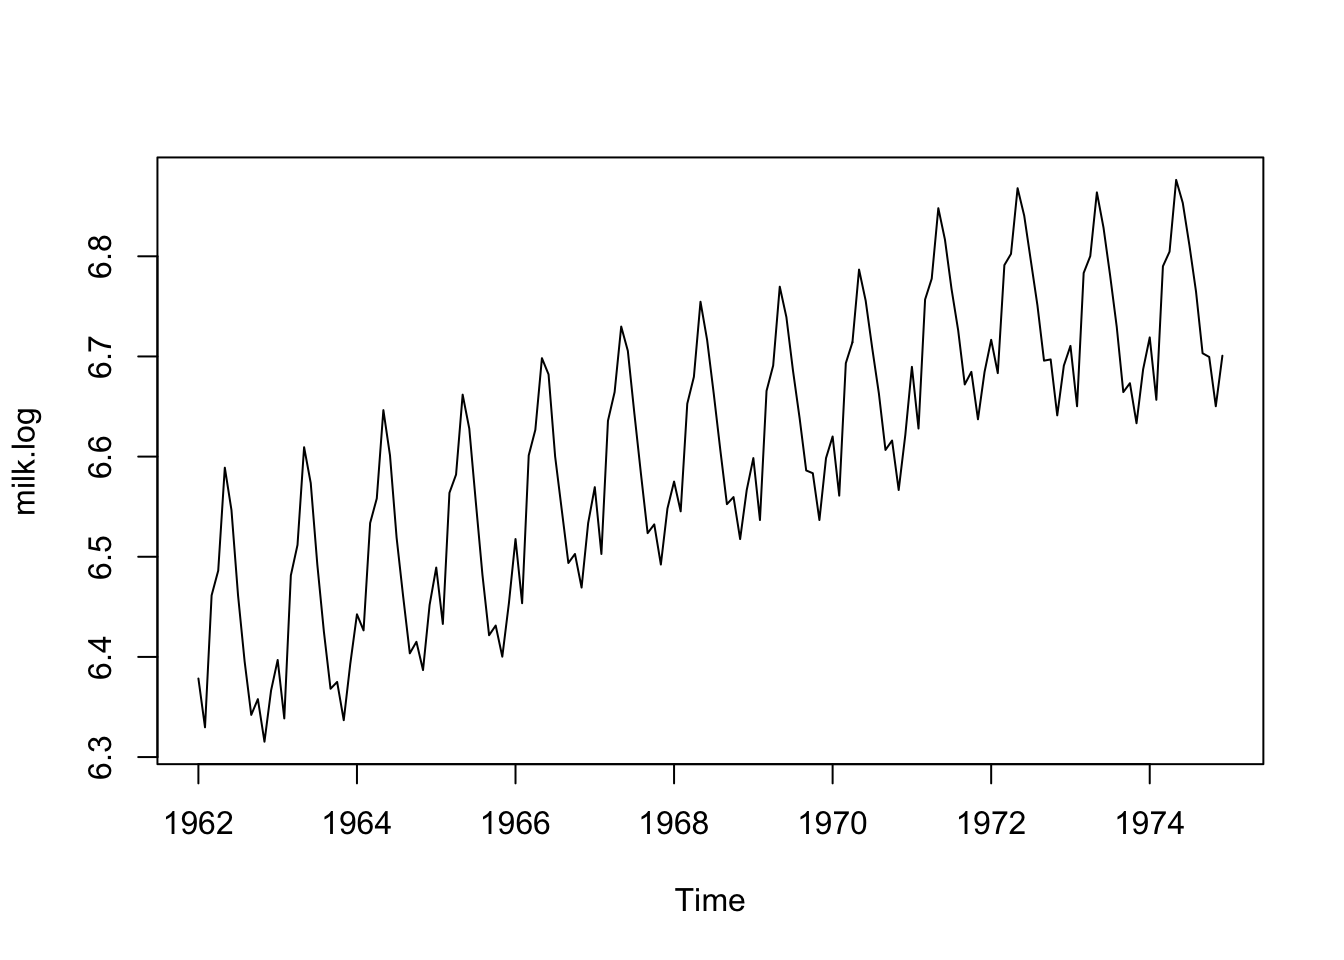
\includegraphics{pstat274_hw02_aoxu_files/figure-latex/unnamed-chunk-6-1.pdf}

\begin{verbatim}
## [1] -0.01762872
\end{verbatim}

\begin{Shaded}
\begin{Highlighting}[]
\SpecialCharTok{{-}}\DecValTok{8}\SpecialCharTok{/}\DecValTok{69}
\end{Highlighting}
\end{Shaded}

\begin{verbatim}
## [1] -0.115942
\end{verbatim}

\begin{Shaded}
\begin{Highlighting}[]
\CommentTok{\# Since {-}0.1424422 is nearly the same as {-}0.115942, then my sample estimate of ρX(2) are nearly the same as its true value found by calculations.}
\end{Highlighting}
\end{Shaded}

\begin{Shaded}
\begin{Highlighting}[]
\NormalTok{xt }\OtherTok{\textless{}{-}} \FunctionTok{arima.sim}\NormalTok{(}\FunctionTok{list}\NormalTok{(}\AttributeTok{ma=}\FunctionTok{c}\NormalTok{(}\DecValTok{1}\NormalTok{,}\DecValTok{2}\NormalTok{,}\SpecialCharTok{{-}}\DecValTok{8}\NormalTok{)),}\AttributeTok{n=}\DecValTok{10000}\NormalTok{)}
\FunctionTok{acf}\NormalTok{(xt, }\AttributeTok{main=}\StringTok{"ACF"}\NormalTok{)}
\FunctionTok{acf}\NormalTok{(xt, }\AttributeTok{main=}\StringTok{"ACF"}\NormalTok{)}\SpecialCharTok{$}\NormalTok{acf[}\DecValTok{3}\NormalTok{]}
\end{Highlighting}
\end{Shaded}

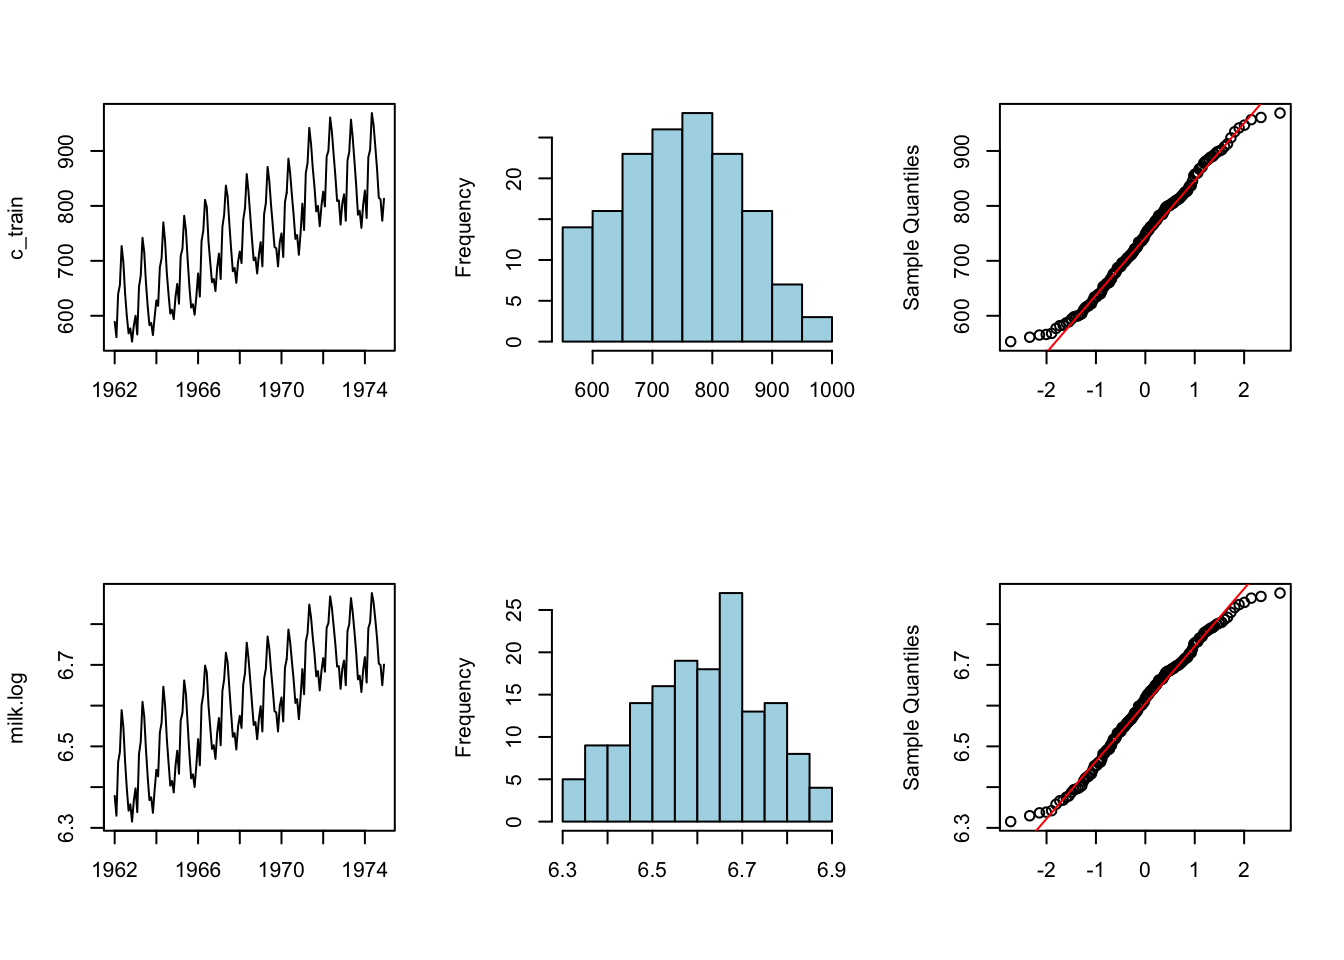
\includegraphics{pstat274_hw02_aoxu_files/figure-latex/unnamed-chunk-7-1.pdf}

\begin{verbatim}
## [1] -0.08658787
\end{verbatim}

\hypertarget{g1}{%
\section{G1}\label{g1}}

\(X_t\) = \(Z_t\) + \(\theta\)\(Z_{t-2}\)

\hypertarget{a-3}{%
\subsection{(a)}\label{a-3}}

E(\(X_t\)\(X_{t+k}\)) =
E((\(Z_t\)+\(\theta\))(\(Z_{t+k}\)\(Z_{t-2+k}\))) =
E(\(Z_t\)\(Z_{t+k}\)) + \(\theta\)E(\(Z_{t-2}\)\(Z_{t+k-2}\)) +
\(\theta\)E(\(Z_{t-2}\)\(Z_{t+k}\)) +
\(\theta^2\)E(\(Z_{t-2}\)\(Z_{t+k-2}\))

\(\gamma_x(t,t+k)\) = E(\(X_t\)\(X_{t+k}\)) - E(\(X_t\))E(\(X_{t+k}\));
When k = 0, \(\gamma_x(t,t+k)\) = 1 + \(\theta^2\); When k = \(\pm2\),
\(\gamma_x(t,t+k)\) = \(\theta\); When k is other numbers,
\(\gamma_x(t,t+k)\) = 0.

Therefore, \(\rho_x(k)\) = 1 when k = 0; \(\rho_x(k)\) =
\(\frac{\theta}{1+\theta^2}\) when k = \(\pm2\); \(\rho_x(k)\) = 0 when
k is other numbers.

When \(\theta\) = 0.8,

Autocovariance function: \(\gamma_x(t,t+k)\) = 1.64 when k = 0;
\(\gamma_x(t,t+k)\) = 0,8 when k = \(\pm2\); \(\gamma_x(t,t+k)\) = 0
when k is other numbers.

Autocorrelation function: \(\rho_x(k)\) = 1 when k = 0; \(\rho_x(k)\) =
\(\frac{20}{41}\) when k = \(\pm2\); \(\rho_x(k)\) = 0 when k is other
numbers.

\hypertarget{b-3}{%
\subsection{(b)}\label{b-3}}

When \(\theta\) = 0.8,

Var(\(\frac{X_1+X_2+X_3+X_4}{4}\)) = \(\frac{Var(X_1+X_2+X_3+X_4)}{16}\)
= \(\frac{1}{16}\)(\((Var(X_1)+Var(X_2)+Var(X_3)+Var(X_4)\) +
2(Cov(\(X_1X_2\))+Cov(\(X_1X_3\))+Cov(\(X_1X_4\))+Cov(\(X_2X_3\))+Cov(\(X_2X_4\))+Cov(\(X_3X_4\))))
= \(\frac{1}{16}\)(4Var(\(X_t\))+4\(\theta\)) =
\(\frac{1}{16}\)(4(\(Var(Z_t)\)+\(\theta^2Var(Z_{t-2})\)+Cov(\(Z_t\),\(Z_{t-2}\)))+4\(\theta\))
= \(\frac{1}{16}\)(4(1+\(\theta^2\))+4\(\theta\)) =
\(\frac{1}{16}\)(4*1.64+3.2) = 0.61

\hypertarget{c-1}{%
\subsection{(c)}\label{c-1}}

When \(\theta\) = -0.8,

Var(\(\frac{X_1+X_2+X_3+X_4}{4}\)) =
\(\frac{1}{16}\)(4(1+\(\theta^2\))+4\(\theta\)) =
\(\frac{1}{16}\)(4*1.64-3.2) = 0.21

The variance in (c) is smaller than in (b) and closer to 0.

\hypertarget{g2}{%
\section{G2}\label{g2}}

Example 1: \(X_t\) = 3\(X_{t-1}\) + 3\(X_{t-2}\) + \(Z_t\)

\begin{Shaded}
\begin{Highlighting}[]
\NormalTok{xt }\OtherTok{\textless{}{-}} \FunctionTok{arima.sim}\NormalTok{(}\FunctionTok{list}\NormalTok{(}\AttributeTok{ma=}\FunctionTok{c}\NormalTok{(}\DecValTok{1}\NormalTok{,}\DecValTok{3}\NormalTok{,}\DecValTok{3}\NormalTok{)),}\AttributeTok{n=}\DecValTok{100}\NormalTok{)}
\FunctionTok{acf}\NormalTok{(xt, }\AttributeTok{main=}\StringTok{"ACF"}\NormalTok{)}
\end{Highlighting}
\end{Shaded}

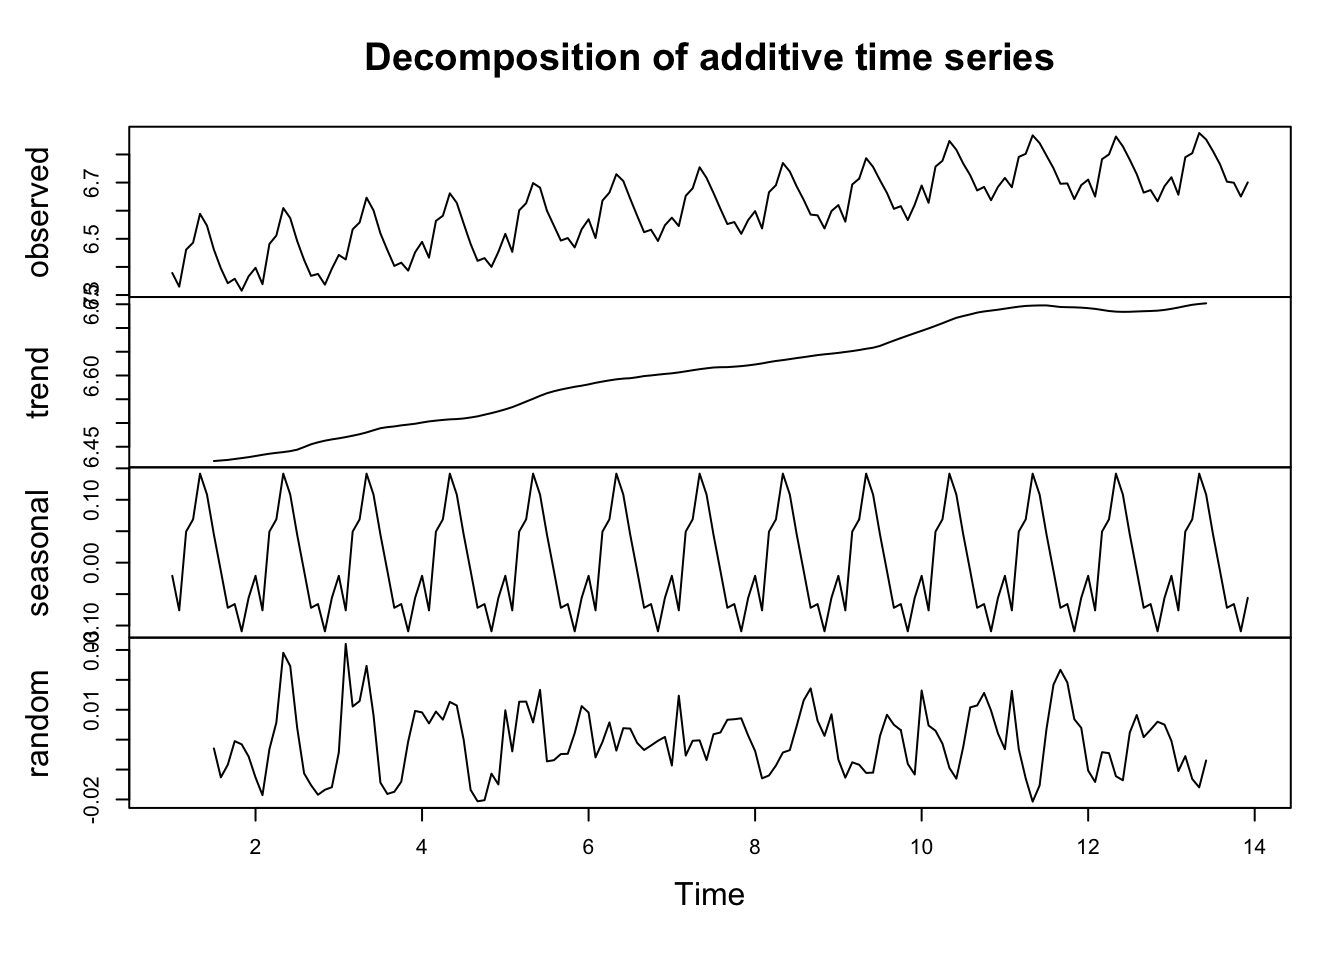
\includegraphics{pstat274_hw02_aoxu_files/figure-latex/unnamed-chunk-8-1.pdf}

\begin{Shaded}
\begin{Highlighting}[]
\FunctionTok{plot}\NormalTok{(xt)}
\end{Highlighting}
\end{Shaded}

\includegraphics{pstat274_hw02_aoxu_files/figure-latex/unnamed-chunk-8-2.pdf}

Example 2: \(X_t\) = 5\(X_{t-1}\) - 8\(X_{t-2}\) + \(Z_t\)

\begin{Shaded}
\begin{Highlighting}[]
\NormalTok{xt }\OtherTok{\textless{}{-}} \FunctionTok{arima.sim}\NormalTok{(}\FunctionTok{list}\NormalTok{(}\AttributeTok{ma=}\FunctionTok{c}\NormalTok{(}\DecValTok{1}\NormalTok{,}\DecValTok{5}\NormalTok{,}\SpecialCharTok{{-}}\DecValTok{8}\NormalTok{)),}\AttributeTok{n=}\DecValTok{100}\NormalTok{)}
\FunctionTok{acf}\NormalTok{(xt, }\AttributeTok{main=}\StringTok{"ACF"}\NormalTok{)}
\end{Highlighting}
\end{Shaded}

\includegraphics{pstat274_hw02_aoxu_files/figure-latex/unnamed-chunk-9-1.pdf}

\begin{Shaded}
\begin{Highlighting}[]
\FunctionTok{plot}\NormalTok{(xt)}
\end{Highlighting}
\end{Shaded}

\includegraphics{pstat274_hw02_aoxu_files/figure-latex/unnamed-chunk-9-2.pdf}

\hypertarget{g3}{%
\section{G3}\label{g3}}

\(E({e}^{\displaystyle \sum_{i=1}^{n}a_ix_i})\) =
E(exp(\(a_1\)(\(Z_1\)+\(\theta\)\(Z_0\))+\(a_2\)(\(Z_2\)+\(\theta\)\(Z_1\))+\ldots+\(a_n\)(\(Z_n\)+\(\theta\)\(Z_{n-1}\))))
=
E(exp(\(a_1\)\(\theta\)\(Z_0\)))E(exp(\(a_1\)+\(a_2\theta\))\(Z_1\)))\ldots E(exp(\(a_n\)\(Z_n\)))
=
m(\(\theta\)\(a_1\))m(\(a_1\)+\(theta\)\(a_2\))\ldots m(\(a_{n-1}\)+\(\theta\)\(a_n\))m\(a_n\)

We find that the MGF of \(x_1\),\(x_2\),\ldots,\(x_n\) depends on
\(a_1\),\(a_2\)\ldots{}\(a_n\) and \(\theta\) but not t, so \(X_t\) is
strictly stationary.

E(\(X_t\)) = E(\(Z_t\)+\(\theta\)\(Z_{t-1}\)) =
E(\(Z_t\))+E(\(\theta\)\(Z_{t-1}\)) = 0 + \(\theta(0)\) = 0;

Cov(\(X_{t+h}\),\(X_t\)) =
Cov(\(Z_{t+h}\)+\(\theta\)\(Z_{t+h-1}\),\(Z_{t}\)+\(\theta\)\(Z_{t-1}\))
= Cov(\(Z_{t+h},Z_t\)) + \(\theta\)Cov(\(Z_{t+h},Z_{t-1}\)) +
\(\theta\)Cov(\(Z_{t+h-1},Z_t\)) +
\(\theta^2\)Cov(\(Z_{t+h-1},Z_{t-1}\)) =
E(\(Z_{t+h}Z_{t}\))+\(\theta\)E(\(Z_{t+h}Z_{t-1}\))+\(\theta\)E(\(Z_{t+h-1}Z_{t}\))+\(\theta^2\)E(\(Z_{t+h-1},Z_{t-1}\))

When h = 0, E(\(Z_t^2\)) = Var(\(Z_t\)) - \(E(Z_t)^2\) = \(\sigma_z^2\),
then Cov(\(X_{t+h}\),\(X_t\)) = \(\sigma_z^2\) +
\(\theta^2\)\(\sigma_z^2\);

When h = \(\pm1\), Cov(\(X_{t+h}\),\(X_t\)) = \(\theta\);

When h is other numbers, Cov(\(X_{t+h}\),\(X_t\)) = 0;

Then, we could get \(\gamma_x(t+h,h)\) = Cov(\(X_{t+h}\),\(X_t\)) =\\
\[\begin{cases} 
  \sigma_Z^2 + \theta^2\sigma_Z^2 & h = 0\\ 
  \theta & h = \pm1\\
  0 & other numbers
\end{cases}\]

Since \(\mu\) is independent of t and \(\gamma_x(t+h,h)\) is also
independent of t, then \(X_t\) is weakly stationary.

Therefore, \(X_t\) is s both weakly and strictly stationary.

\end{document}
